\section{\bi{Global phase diagram on a width strip}{連續寬度條帶上的全域相圖}}
\begin{thm}\label{th:strip}
\bi{For $N=6$, $7.99\le s\le9$ and $0<h\le1/6$, every global minimizer has, up to cyclic starting point, the gaps of \eqref{eq:y} with a displacement in Table~\ref{tab:phases}. For $8\le s\le9$, $\Delta=h_b-h_c$ satisfies $0.000209555<\Delta'(s)<0.000734655$. In the collision closure at $h=0$, for $8\le s\le9$ all minimizers reduce to an antipodal opposite-charge pair; two neutral coincident pairs can be placed anywhere consistent with cyclic alternation.}{當 $N=6$、$7.99\le s\le9$、$0<h\le1/6$，全部全域極小者的間隙字皆為式 \eqref{eq:y} 所對應間隙字的循環移位，位移取表~\ref{tab:phases} 所列值。在 $8\le s\le9$，$\Delta=h_b-h_c$ 滿足 $0.000209555<\Delta'(s)<0.000734655$。在同一 $[8,9]$ 上令 $h=0$ 並容許碰撞，則全部極小者抵消後剩下一對異號對徑粒子；另兩對同點中性粒子可放於任何保持循環交替次序的位置。}
\end{thm}
\begin{proof}
\bi{\emph{Small floors.} We give the two sets of estimates together. Use $\Q=\sum a_n|P_n|^2$, $T_p^*=\sum_{n\ge3}n^p a_n$. For the broad strip $[8,9]$ and $h\le .07$, put $r=.335$, $e=.44$; for the narrow strip $[7.99,8.01]$ and $h\le .10$, put $r=.292$, $e=\pi/5$. Then $q<r$ and $\eta\le e$. The degree-eight positive Taylor lower bound for $\exp(3.1415^2/8.01)$ suffices at the narrow right endpoint, the degree-seven bound for $\exp(3.14^2/9)$ at the broad one. Projection of $P_n=-in\int_A e^{inu}\dd u$ onto its phase gives $|P_n|\le\min(2n,6)$. Bound $T_p^*\le3^p r^8/[1-(4/3)^p r^7]$ for $p=2,3,4$. Comparing with the centered triples gives $|P_1|^2\ge4(2\cos\eta-1)^2-(16q^3+4T_2^*)$. The following constants apply in the two cases.}{\emph{小間距。} 將兩個寬度段的估計並列。記 $\Q=\sum a_n|P_n|^2$、$T_p^*=\sum_{n\ge3}n^pa_n$。廣帶 $[8,9]$ 且 $h\le .07$ 時取 $r=.335$、$e=.44$；窄帶 $[7.99,8.01]$ 且 $h\le .10$ 時取 $r=.292$、$e=\pi/5$。均有 $q<r$、$\eta\le e$。在窄帶右端以 $\exp(3.1415^2/8.01)$ 的八階正 Taylor 下界核對，在廣帶右端以 $\exp(3.14^2/9)$ 的七階下界核對。將 $P_n=-in\int_A e^{inu}\dd u$ 投影至自身方向得 $|P_n|\le\min(2n,6)$。對 $p=2,3,4$ 有 $T_p^*\le3^p r^8/[1-(4/3)^p r^7]$。與居中三簇比較得 $|P_1|^2\ge4(2\cos\eta-1)^2-(16q^3+4T_2^*)$。兩組常數如下。}
\[
\begin{array}{c|ccccc}
 r &16q^3+4T_2^* &16q^3+10T_2^* &32q^3+10T_3^*&R & |P_1|\\\hline
 .335 &<.608&<.616&<1.246&<.615&>1.41\\
 .292 &<.405&<.41&<.82&<.41&>1.055
\end{array}
\]
\bi{A maximal packed block ends at slack gaps. Rotate $P_1$ to the positive real axis and freeze $V(u)=\sum a_n\operatorname{Re}(\overline{P_n}e^{inu})$ at a maximizer $X$. In comparing to $Y$ the difference of $\Q$ equals the change in $2\sum\sigma_iV$ plus $\sum a_n|P_n(Y)-P_n(X)|^2$. Hence each independently movable block locally maximizes its fixed-potential score. For lengths $1,2,3,4$ the harmonic multipliers for odd-block cosine or even-block sine are $1,2\sin(w/2),2\cos w-1,4\cos w\sin(w/2)$ at $w=n\eta$. Divide by their positive first-mode factors. The multiplier ratio in modulus is at most 2 for $n=2$ and $5n/3$ thereafter, by the sine multiple inequality and $2\cos\eta-1>.6$. Thus the middle two derivative bounds above control the first and second derivative remainders. The first-mode peak for positive odd, positive even, negative odd and negative even blocks is at $0,\pi/2,\pi,3\pi/2$ respectively. Stationarity and nonpositive curvature confine their midpoints within $d=.46$ (broad) or $.42$ (narrow) of their own peak: the derivative remainder is below $|P_1|\sin d$ and the curvature remainder below $|P_1|\cos d$.}{極大緊塊的兩側均為鬆弛間隙。將 $P_1$ 旋至正實軸，在極大者 $X$ 固定 $V(u)=\sum a_n\operatorname{Re}(\overline{P_n}e^{inu})$。由 $X$ 至 $Y$ 的 $\Q$ 變化等於 $2\sum\sigma_iV$ 的變化加 $\sum a_n|P_n(Y)-P_n(X)|^2$，所以可獨立平移的每一塊都局部極大化固定勢得分。對長度 $1,2,3,4$ 的塊，其奇塊餘弦、偶塊正弦的模態乘子在 $w=n\eta$ 依次為 $1,2\sin(w/2),2\cos w-1,4\cos w\sin(w/2)$。各自除以正的一階乘子，由正弦倍角界及 $2\cos\eta-1>.6$，其絕對比值在 $n=2$ 至多為二，其後至多 $5n/3$。故上表導數兩欄分別控制一、二階餘項。正奇、正偶、負奇、負偶塊的第一模峰位依次為 $0,\pi/2,\pi,3\pi/2$。一階駐點與非正曲率使中點距各自峰位至多 $d=.46$（廣帶）或 $.42$（窄帶），因一階餘項小於 $|P_1|\sin d$，二階餘項小於 $|P_1|\cos d$。}

\bi{With at least three blocks, each has size at most four. Odd blocks alternate in sign and their two disjoint arcs cannot be visited alternately twice around the circle. An even block between a positive and the following negative odd block would have negative initial sign and a peak in the complementary arc. The reverse arc likewise excludes positive even blocks. Thus odd blocks, when present, leave only two blocks. For all-even blocks in the broad case, the three constituent dimers give $|P_1|\le3\eta<1.32$. In the narrow case a single length-six block has $|P_1|=|\sin(3\eta)|/\cos(\eta/2)<1.055$. Otherwise all even blocks start with the same sign in one arc of length $.84$. For $\eta\le.30$, $3\eta<1.055$. For larger $\eta$ a $4+2$ pair has midpoint spacing at least $3\eta$, and three dimers span at least $4\eta$, both exceeding $.84$. Only $5+1$ or $3+3$ remains.}{若至少三塊，則每塊至多四粒子。奇塊的起始符號交替，環繞一週不可能兩度交替經過兩個不交峰區。若正奇塊至下一負奇塊間出現偶塊，它必以負號開始，但峰位在另一段弧上。反向的弧同理排除正偶塊。因此若有奇塊，只剩兩塊。全偶分簇在廣帶可分作三對緊偶極，故 $|P_1|\le3\eta<1.32$。在窄帶，單一六粒子塊有 $|P_1|=|\sin(3\eta)|/\cos(\eta/2)<1.055$。其餘全偶分簇的起始符號一致，中點皆處於長 $.84$ 的弧內。若 $\eta\le .30$，則 $3\eta<1.055$；若更大，$4+2$ 的中點至少相隔 $3\eta$，三個二粒子塊的中點跨度至少 $4\eta$，均超出 $.84$。僅餘 $5+1$ 或 $3+3$。}

\bi{Put $A(w)=2\cos w-1$, $B(w)=1-2\cos w+2\cos(2w)$, and $D_1(w)=4\sin^2 w\, A(w)^2=4A(w)^2-(1+B(w))^2$. For a shift $v$ in angle, $1-\cos(nv)\le n^2(1-\cos v)$. On the broad strip the centered $5+1$ gains at least $2(1-\cos v)[B(\eta)-4q^3-5T_2^*]$ against its shift, with bracket $>.26$: $|B(2\eta)|\le1$ since $B(w)=\cos(5w/2)/\cos(w/2)$ and $2\eta<\pi/3$. Against the centered unequal split the triples gain at least $D_1(\eta)-9R\eta^4>1.36\eta^2$, since all odd-mode differences $D_1(n\eta)$ are nonnegative and $|B(w)-1|\le3w^2$. On the narrow strip for $\eta\le .40$ use instead $B(\eta)-5R/4>0$ and the same lower bound $D_1(\eta)-9R\eta^4>0$ (use $\sin\eta\ge\eta(1-\eta^2/6)$). For $.40\le\eta\le\pi/5$, $B(\eta)\ge0$ and $D_1(\eta)>.405$ beats the entire high-mode score for every placement: as a function of $\cos\eta$ its minimum on $[.8,.922]$ occurs at an endpoint. Theorem~\ref{th:face} now centers the surviving triples.}{記 $A(w)=2\cos w-1$、$B(w)=1-2\cos w+2\cos(2w)$、$D_1(w)=4\sin^2 w\,A(w)^2=4A(w)^2-(1+B(w))^2$。角位移 $v$ 滿足 $1-\cos(nv)\le n^2(1-\cos v)$。廣帶上，居中 $5+1$ 比偏移者至少多得 $2(1-\cos v)[B(\eta)-4q^3-5T_2^*]$，括號 $>.26$；此處 $B(w)=\cos(5w/2)/\cos(w/2)$ 且 $2\eta<\pi/3$，故 $|B(2\eta)|\le1$。對居中不等分簇，雙三簇至少多得 $D_1(\eta)-9R\eta^4>1.36\eta^2$，因奇模差 $D_1(n\eta)$ 均非負，且 $|B(w)-1|\le3w^2$。窄帶上對 $\eta\le .40$ 改用 $B(\eta)-5R/4>0$ 及 $D_1(\eta)-9R\eta^4>0$（用 $\sin\eta\ge\eta(1-\eta^2/6)$）。若 $.40\le\eta\le\pi/5$，則 $B(\eta)\ge0$ 且 $D_1(\eta)>.405$ 已超過任意擺位的高模總得分；將其視為 $\cos\eta$ 的函數，在 $[.8,.922]$ 上的最低值出現於端點。再由定理~\ref{th:face} 選出留下之雙三簇的居中位置。}

\bi{\emph{All remaining floors.} The exhaustive certificate in Appendix~\ref{sec:cert} shows that every maximizer lies on the closed face \eqref{eq:y} throughout $[.10,1/6)$ on the narrow strip and $[.07,1/6)$ on the broad strip. The two reductions overlap at their junctions. All widths here have $q<17/50$, so Theorem~\ref{th:face} completes the global classification. At $h=1/6$ feasibility alone suffices. In the collision closure $R\le .615$ on $[8,9]$, so the equality argument following \eqref{eq:deficit} proves the assertion, including arbitrary placement of the neutral pairs.}{\emph{其餘下限。} 附錄~\ref{sec:cert} 的窮盡證書證明：窄帶的 $[.10,1/6)$ 及廣帶的 $[.07,1/6)$ 上，極大者全部位於閉面 \eqref{eq:y}。各歸約在接合處重疊。兩帶均有 $q<17/50$，故定理~\ref{th:face} 完成全域分類。$h=1/6$ 直接由可行性決定。在 $[8,9]$ 有 $R\le .615$，碰撞閉包的取等遂由式 \eqref{eq:deficit} 之後的論證得到，亦允許中性對自由放置。}

\bi{\emph{Separation of the curves.} Split $[8,9]$ into 32 closed intervals. In each, monotonicity encloses both roots using rational bisection at the endpoints. In \eqref{eq:slope} evaluate $h'=-P_q(\pi^2 q/s^2)/[-2\pi\sqrt{1-x^2}\,P_x]$ over each root box, including $z'(x)$ in $P_x$ for outer contact. Enclose the polynomial parts by the Chebyshev recurrences and their differentiated recurrences; use the same tails as in Theorem~\ref{th:face} from the first omitted frequency. To retain their common dependence on width, enclose the fractions $qP_q/[\sqrt{1-x^2}\,P_x]$ separately, subtract the centered fraction from the contact fraction, and only then multiply the interval difference by the common positive factor $\pi/(2s^2)$. All 32 intervals lie strictly inside the stated bounds. Hence the minimum and maximum of $\Delta$ on the strip $[8,9]$ occur uniquely at 8 and 9, respectively. Integer endpoint tests give Table~\ref{tab:roots}; independent image sums check both signs at each of its twenty endpoints.}{\emph{兩相界的間距。} 將 $[8,9]$ 分成 32 個閉區間，在每段兩端以有理二分求根，利用單調性包住整段的兩根。於各根盒以式 \eqref{eq:slope} 計算 $h'=-P_q(\pi^2 q/s^2)/[-2\pi\sqrt{1-x^2}\,P_x]$，外接觸的 $P_x$ 包含 $z'(x)$。利用 Chebyshev 遞推及其微分遞推包住多項式，從首個略去的頻率起採定理~\ref{th:face} 所用的尾項估計。為保留兩根共同的寬度依賴，分別包住分式 $qP_q/[\sqrt{1-x^2}\,P_x]$，先以外接觸分式減去中央分式，最後才將差區間乘以共同正因子 $\pi/(2s^2)$；32 段的上下界皆嚴格落在定理所述界內。故在 $[8,9]$，$\Delta$ 的最小與最大值分別僅在 8 與 9 取得。有理端點判號給出表~\ref{tab:roots}，另以獨立像和復核二十個端點的符號。}
\bi{Specializing the same implicit derivatives at $s=8$ and using the narrow root enclosures gives}{在 $s=8$ 處代入較窄的根包圍並計算同一隱導數，可得}
\begin{align*}
 -.004653798&<h_c'(8)<-.004653797,\\
 -.004095783&<h_b'(8)<-.004095782,\\
 .0005580150&<\Delta'(8)<.0005580151 .
\end{align*}
\end{proof}
\par
\begin{table}[tbp]\centering
\caption{\bi{Each integer $k$ encloses the named root strictly between $k\,10^{-17}$ and $(k+1)10^{-17}$.}{每個整數 $k$ 表示相應根嚴格介於 $k\,10^{-17}$ 與 $(k+1)10^{-17}$。}}\label{tab:roots}
\begin{tabular}{r rr}\toprule $s$ & $k_c$ & $k_b$\\\midrule
8&13114680495074862&13327908477025674\\
8.25&13002116216464920&13228696963489349\\
8.5&12896949017617399&13135593571511805\\
8.75&12798925229764372&13048218048706585\\
9&12707787492004334&12966203092650766\\\bottomrule
\end{tabular}\end{table}
\par
\begin{figure}[htbp]\centering
\ifChinese
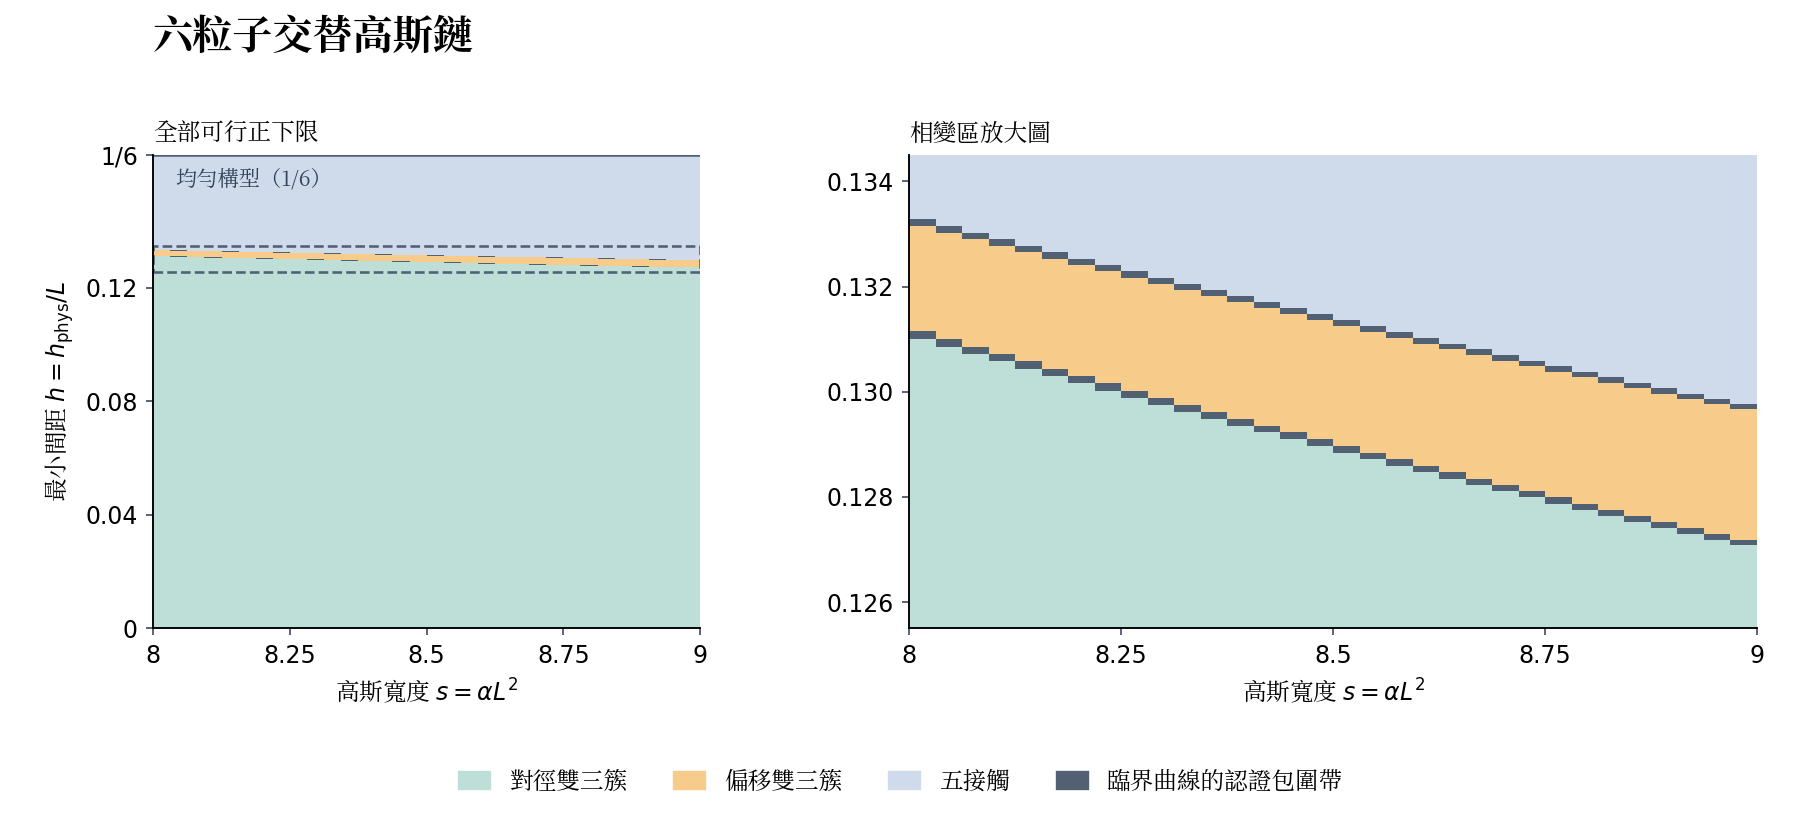
\includegraphics[width=.98\linewidth]{../../research/six-site/width-strip-zh.png}
\else
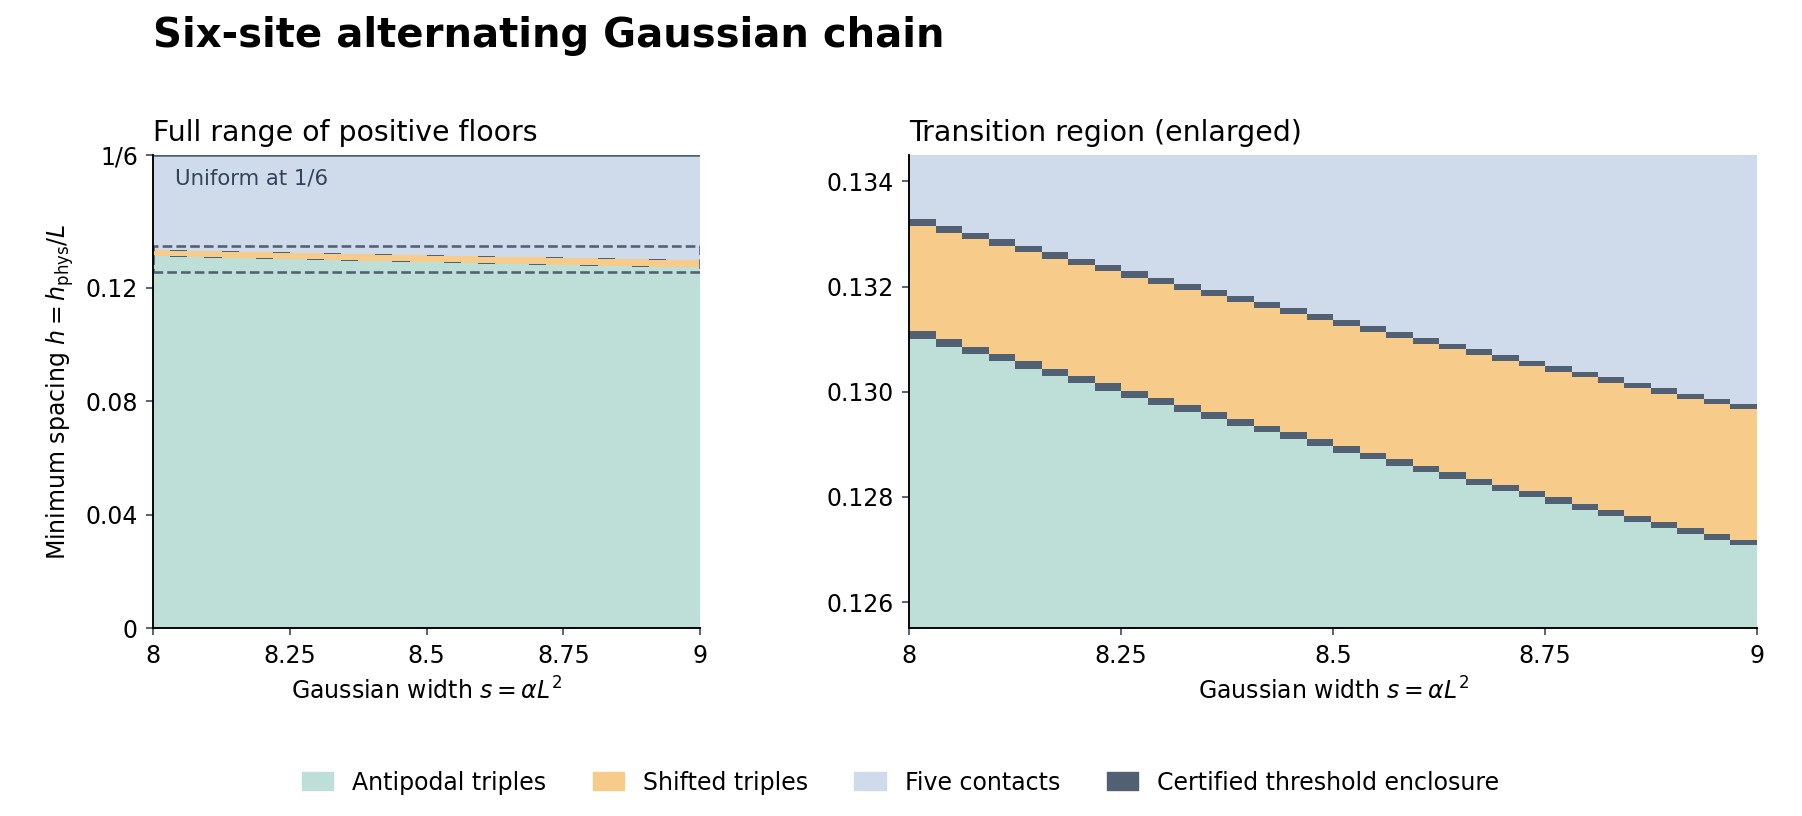
\includegraphics[width=.98\linewidth]{../../research/six-site/width-strip.png}
\fi
\caption{\bi{Global minimizers on $[8,9]$ and an enlargement of the transition region. Green denotes centered, orange shifted, and blue five-contact cells. Dark steps enclose the true curves by monotonicity between consecutive certified endpoints at spacing $1/32$. At $h=1/6$ the cell is uniform.}{寬度 $[8,9]$ 上的全域極小者與相變區放大圖。綠、橙、藍分別為對徑、偏移及五接觸相。相距 $1/32$ 的認證端點及單調性給出深色階梯包圍帶。$h=1/6$ 時構型均勻。}}\label{fig:strip}
\end{figure}

